\documentclass[handout,usenames,dvipsnames]{beamer}
\usefonttheme{structurebold}       % bold headings
\usefonttheme{professionalfonts}   % fancier equations
\usetheme{Warsaw}
\usepackage[utf8]{inputenc} 
\usepackage[ngerman]{babel} 
\usepackage{mathtools}
\usepackage{stmaryrd}
\usepackage{framed}
\usepackage{tabu}
\usepackage{marvosym}
\usepackage{multicol}

\setbeamertemplate{footline}[frame number]{}

\newcounter{sauvegardeenumi}
\newcommand{\asuivre}{\setcounter{sauvegardeenumi}{\theenumi}}
\newcommand{\suite}{\setcounter{enumi}{\thesauvegardeenumi}}

\begin{document}

\title{Untersuchung der Anwendung homomorpher Kryptosysteme unter Berücksichtigung der unautorisierten Verformbarkeit von Chiffretexten}  
\author{\texorpdfstring{
		Matthias Ulbrich\newline
		 \url{matt@uni-bonn.de}}{Matthias Ulbrich}\newline
		 2743974}

\date{21. Juni 2017} 

%\titlegraphic{
\includegraphics[width=1cm]{fig/unilogo}}


	
\begin{frame}
\titlepage
\end{frame} 
	
\begin{frame}
\frametitle{Übersicht}
\tableofcontents
\end{frame} 
	
\section{Einleitung} 

\begin{frame}
\frametitle{Einleitung} 
\begin{itemize}
	\item 	Homomorphe Kryptosysteme sind eine Erweiterung klassischer Kryptosysteme
	\item	Sie unterscheiden sich durch: Sicherheitseigenschaften gegenüber Angreifermodellen, möglichen homomorphe Rechenoperationen, Chiffretextexpansion, Performance (Anzahl der Rechenschritte)
\end{itemize}
\textbf{Ziel:} Wir möchten eine Empfehlung für folgende Frage abgeben können.\\
\textbf{Frage:} Bob möchte ein Wasserzeichen in einem verschlüsselten Bild einbetten. Welches homomorphe Kryptosystem sollte er verwenden?
\end{frame}

\section{Grundlegende Aspekte}
\subsection{Homomorphes Kryptosystem}

\begin{frame}
	\frametitle{Kryptosystem}
	Ein Kryptosystem besteht aus fünf Mengen mit drei auf ihnen anwendbaren Algorithmen:
	\begin{block}{Kryptosystem K}
		\begin{itemize}
			\item K ist Quintupel der Mengen: $K = (\mathcal{P},\mathcal{C},\mathcal{K},\mathcal{E},\mathcal{D})$
			\item Für alle Schlüssel $k\in \mathcal{K}$ gibt es Funktionen  $\mathcal{E}\ni e_k:\mathcal{P}\rightarrow\mathcal{C}$ und  $\mathcal{D}\ni d_k:\mathcal{C}\rightarrow\mathcal{D}$, so dass für alle Klartexte $x\in\mathcal{P}$ folgende Identität gilt: 
			\begin{equation*} d_k(e_k(x)) = x. \end{equation*}
		\end{itemize}
	\end{block}
\end{frame}

\begin{frame}
	\frametitle{Homomorphes Kryptosystem} 
	Erweiternde Eigenschaften:
	\begin{itemize}
		\item \textbf{asymmetrisch}: Durchführung von Rechenoperationen zusätzlich zu einer einfachen Verschlüsselung durch Kenntnis des öffentlichen Schlüssels.
		\item \textbf{probabilistisch}: Die Anwendung der Verschlüsselungsfunktion wird durch Zufallszahlen nicht-deterministisch:
		\begin{equation*} e_{k_p}(x,r) \neq e_{k_p}(x,r'). \end{equation*}
		\item (semihomomorph) Verschlüsselungsfunktion ist ein \textbf{Gruppenhomomorphismus} der Gruppen $(\mathcal{P},\oplus), (\mathcal{C},\odot)$. Für Chiffretexte  $e_{k_p}(x_1)=c_1$, $e_{k_p}(x_2)=c_2$ gilt:	
		\begin{equation*}   d_{k_s}(c_1\odot c_2)= x_1\oplus x_2.	\end{equation*}
	\end{itemize}
\end{frame}

\begin{frame}
	\frametitle{Beispiel: Okamoto-Uchiyama Kryptosystem}
%	\textbf{Schlüsselgenerierung}: 
%	\begin{enumerate}
%		\item Wähle zwei große Primzahlen $p,q\ (|p|=|q|=k)$.
%		\item Wähle $g\in(\mathbb{Z}/ n\mathbb{Z})^*$, so dass für die Ordnung $g_p$ von $g$ gilt: $g_p \coloneqq g^{p-1}\ \text{mod}\ p^2 \stackrel{!}{=} p$
%		\item Setzte $n=p^2 q$ und $h=g^n\ \text{mod}\ n$.
%	\end{enumerate}
    öffentlicher Schlüssel $(n,g,h)$, privater Schlüssel $(p,q)$ \newline
    
    \textbf{Verschlüsselung}:
    \begin{equation*}    e(m,r)=g^m h^r\ \text{mod}\ n \text{  mit gleichverteiltem  } r\in(\mathbb{Z}/ n\mathbb{Z}) \end{equation*}
    
    \textbf{Homomorphe Addition}:
    \begin{align*}
    e(m_1,r_1) e(m_2,r_2)\ \text{mod}\ n &= g^{m_1} h^{r_1}g^{m_2} h^{r_2} \ \text{mod}\ n  \\ & =  g^{m_1+m_2} h^{r_3}\ \text{mod}\ n \\ &= e(m_1+m_2,r_3) \ \text{mod}\ n\  
    \end{align*}
    
    \textbf{Homomorphe Multiplikation}:
    \begin{equation*}
    e(m, r)^k = (g^{m} h^{r})^k \ \text{mod}\ n = g^{m k} h^{r'}\ \text{mod}\ n = e(m k, r') \text{mod}\ n
    \end{equation*}
   
	
\end{frame}

\subsection{Sicherheitseigenschaften}
\begin{frame}
	\frametitle{Sicherheitsziele}
	\begin{itemize}
		\item 	\textbf{Ununterscheidbarkeit von Chiffretexten (IND)}: Geben ein Chiffretext $c_b$ von \textit{einem} der Klartexte $x_1, x_2$. Der Angreifer soll $b=?$ nicht besser als ein zufällig ratender Angreifer ermitteln können.\newline
%	\begin{equation*}	\text{Adv}_\mathcal{A} = \left| Pr\left(\mathcal{A}(\text{ermitteln},c_b,k_p,x_1,x_2)=b\right)-\frac{1}{2}  \right|.\end{equation*}
	\item \textbf{Keine unautorisierte Verformbarkeit (NM)}:
	Der Angreifer will einen Chiffretext $c$ von Klartext $x$ zu einem Chiffretext $c'$ gezielt verformen. Dabei soll $c'$ in einer gewünschten Beziehung zu $x$ stehen (formal: $\mathcal{R}(x,x')$). Der Angreifer soll $c'$ nicht besser ermitteln können als wäre es zufällig erzeugt. \newline
		\end{itemize}
	
	Hier verfügt der Angreifer über den öffentlichen Schlüssel für seinen Angriff. $\rightarrow$ Grundsätzlich möglich: CPA1-Angriff.
	
\end{frame}

%\begin{frame}
%	\frametitle{Sicherheitsziele unter verschiedenen Angreifermodellen}
%	Der Angreifer erhält neben dem öffentlichen Schlüssel, ein \textit{Entschlüsselungsorakel} welches ihm Klartexte zu gegebenen Chiffretexten zurück gibt. $\rightarrow$ CPA2-, CCA1-, CCA2-Angriff\newline
	
%	Dies führt zu den Sicherheitseigenschaften: 
%	\begin{figure}
%		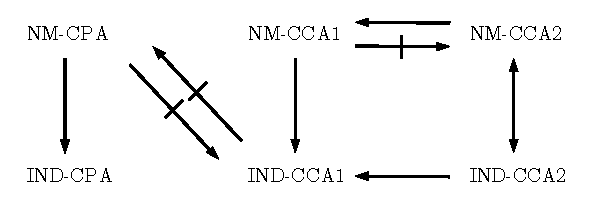
\includegraphics[]{fig/Implikationen.pdf} 
%	\end{figure}
%\end{frame}

\section{Sicherheit homomorpher Kryptosysteme}
\begin{frame}
	\frametitle{Sicherheit homomorpher Kryptosyteme} 
	\begin{block}{Relevante kryptografische Angreifer}
	\begin{enumerate}
		\item Asymmetrie\\ $\rightarrow$ mindestens nötig: Sicherheit vor IND-CPA1-Angreifern.
		\item Homomorphieeigenschaft impliziert unautorisierte Verformbarkeit\\ $\rightarrow$ höchstens möglich: Sicherheit vor IND-CCA1-Angreifern.
	\end{enumerate}
	\end{block}

	Wie wird eine Integrität von Rechenoperationen beim Einsatz homomorpher Kryptosysteme gewährleistet? 
\end{frame}

\section{Untersuchte Veröffentlichungen}
\subsection{Untersuchte Kriterien für die Klassifizierung}
\begin{frame}
	\frametitle{Untersuchte Kriterien für die Klassifizierung}
	Um Bob eine Empfehlung geben zu können sollen Auswahlkriterien eines Kryptosystems identifiziert werden:
	\begin{itemize}
		\item besondere Eigenschaften des Kryptosystems
		\item realisierte Berechnungen im Chiffreraum
		\item Umgang mit unautorisierter Verformbarkeit der Chiffretexte: Wie wird eine Integrität der Chiffretexte gewährleistet?
	\end{itemize}
\end{frame}

\subsection{Untersuchung von Autocrypt \cite{tople2013autocrypt} }
\begin{frame}
	\frametitle{Untersuchung von Autocrypt \cite{tople2013autocrypt} }
	\begin{figure}
		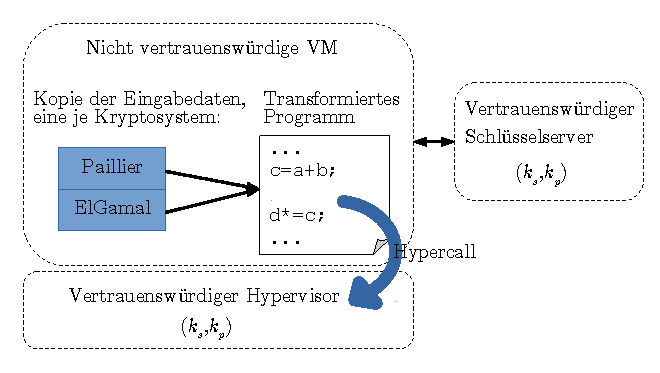
\includegraphics[]{fig/Autocrypt.pdf} 
	\end{figure}
\end{frame}

\begin{frame}
	\textbf{Klassifizierungskriterien:}
	\begin{enumerate}
		\item Paillier, ElGamal sind IND-CPA sicher $\rightarrow$ Transformiertes Programme ist IND-CPA sicher.\newline Zwei semihomomorphe Kryptosysteme in Kombination, da dies effizienter ist als die Verwendung \textit{eines} vollhomomorphen Kryptosystems. 
		\item Das Paillier Kryptosystem wird eingesetzt, um homomorphe Bitoperationen zu ermöglichen.
		\item Eine Integrität der Rechenoperationen wird ausdrücklich nicht berücksichtigt.
	\end{enumerate}
\end{frame}

\subsection{Untersuchung von Privacy Preserving Face Recognition \cite{erkin2009privacy}}
\begin{frame}
	\frametitle{Untersuchung von Privacy Preserving Face Recognition \cite{erkin2009privacy}}
	\begin{figure}
	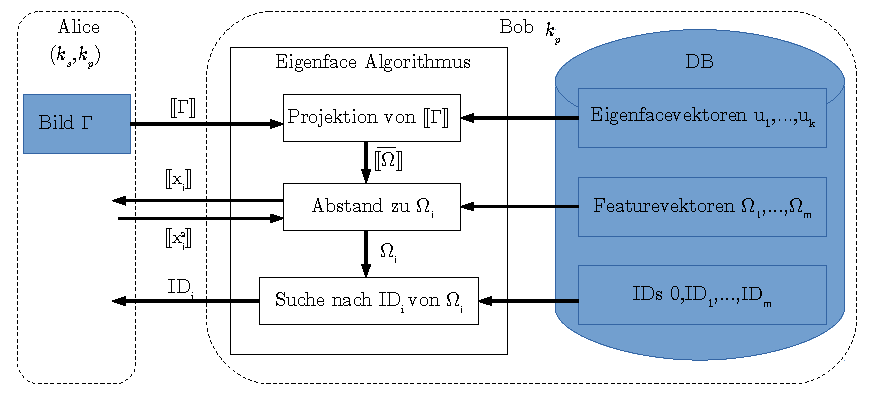
\includegraphics[scale=0.7]{fig/Faces.pdf} 
	\end{figure}
\end{frame}

\begin{frame}
	\textbf{Klassifizierungskriterien:}
	\begin{enumerate}
		\item Einsatz mehrerer Kryptosysteme zur Optimierung der Performance: Paillier (schnelle Schlüsselgenerierung, Vorberechnungen),  DGK für schnelle Vergleiche.
		\item Projektion (Skalarprodukt), quadratischer Abstand, jedoch nur möglich unter besonderen Vorraussetzungen des Anwendungsfalls.
		%Diese Berechnungen sind allerdings nur möglich, weil eine der Zahlen unverschlüsselt in die Berechnung eingeht. Weiter wird bei beim quadratischen Abstand auf das Wurzelziehen verzichtet, da man nur an einem relativen Vergleich der Ergebnisse interessiert ist.
		\item  unautorisierte Verformbarkeit nicht ausnutzbar: ein verformter Chiffretext wird im Protokoll nicht mehr zurück erhalten und der Angreifer kontrolliert höchstens eine Partei 
	\end{enumerate}
\end{frame}

\section{Klassifikation}

\begin{frame}
	\frametitle{Anwendungsfälle homomorpher Kryptosysteme 1/2}
	%\begin{center}
		\tiny
		\begin{tabu}{ | l | p{3.2cm} |  p{1cm} |  p{3.7cm} |}
			
			\hline
			\textbf{Veröffentlichung} & \textbf{Kryptosystem (Implementierung)} & \textbf{Angreifer} & \textbf{Integritätsprüfung der Chiffretexte} \\ \hline  \tabucline[1pt]{-}
			
			\cite{tople2013autocrypt} 
			& ElGamal (libcrypt \cite{libcrypt:online}),
			\newline Paillier (CryptDB \cite{popa2011cryptdb})
			& Bösartig
			& Nein, ausdrücklich nicht berücksichtigt \\ \hline
			
			\cite{bost2015machine} 
			& Goldwasser-Micali, Paillier\newline (jeweils eigene Implementierung \cite{ciphermed:online} in C++ mit GMP \cite{gmp:online} und NTL \cite{nlt:online}), BGV (HElib \cite{HElib:online}\cite{halevi2013design})
			& HBC 
			& Nein\\ \hline
			
			\cite{nikolaenko2013privacy}
			& Hash-ElGamal (eigene Implementierung)
			& Bösartig
			& \textbf{Signierung mit MAC-Code}  \\ \hline
			
			\cite{damgaard2007efficient}
			& DGK (eigene Implementierung in Java 1.5 unter Verwendung der Klasse BigInteger)
			& HBC
			& Nein \\ \hline
			
			\cite{kuribayashi2005fingerprinting}
			& Okamoto-Uchiyama (eigene Implementierung %\footnote{Die Autoren haben die Algorithmen des Kryptosystems selber implementiert. Der Quellcode ist nicht veröffentlicht.}
			)
			& HBC
			& unautorisierte Verformbarkeit nicht ausnutzbar: ein verformter Chiffretext wird im Protokoll nicht mehr zurück erhalten und der Angreifer kontrolliert höchstens eine Partei \\ \hline
			
			\cite{erkin2009privacy} 
			& Paillier, DGK (jeweils eigene Implementierung mit kryptografischen Optimierungen aus \cite{damgaard2001generalisation} in C++ mit GMP \cite{gmp:online})
			& HBC
			& Nicht ausnutzbar im HBC Modell, da nicht vom Protokoll abgewichen wird. \\ \hline
			
			\cite{bos2014private}	
			& BLLN (eigene Implementierung mit kryptografischen Optimierungen aus \cite{brakerski2012fully})
			& HBC
			&  unautorisierte Verformbarkeit nicht ausnutzbar: ein verformter Chiffretext wird im Protokoll nicht mehr zurück erhalten und der Angreifer kontrolliert höchstens eine Partei\\ \hline
		\end{tabu}
	%\end{center}
\end{frame}	

\begin{frame}
	\frametitle{Anwendungsfälle homomorpher Kryptosysteme 2/2}
	\tiny
	\begin{tabu}{ | l | p{3cm} |p{3cm}|}
		\hline
		\textbf{Veröffentlichung} & \textbf{Chiffretextwechsel} & \textbf{Grund für Chiffretextwechsel}\\ \hline  \tabucline[1pt]{-}
		
		\cite{tople2013autocrypt} 
		& ElGamal $\leftrightarrow$ Paillier
		& Durchführung von Addition und Multiplikation mit gleicher Variable \\ \hline
		
		\cite{bost2015machine}
		& Goldwasser-Micali $\rightarrow$ BGV
		\newline  Goldwasser-Micali  $\rightarrow$ Paillier 
		&  Evaluierung von Polynomen,
		\newline Weiterrechnen unter Paillier\\ \hline	
		
		\cite{nikolaenko2013privacy}
		& -
		& - \\ \hline
		
		\cite{damgaard2007efficient} 
		& -
		& -\\ \hline	
		
		\cite{kuribayashi2005fingerprinting}
		& - 
		& - \\ \hline
		
		\cite{erkin2009privacy}  
		& Paillier $\rightarrow$ DGK
		& schnellere Vergleiche\\ \hline
		
		\cite{bos2014private}	 
		& -
		& - \\ \hline
	\end{tabu}
\end{frame}

\begin{frame}
	\frametitle{Auswahlkriterien homomorpher Kryptosysteme}
	 \tiny
	\begin{tabu}{ | l |p{3cm} | l | p{1cm} | l |}
		\hline
		\textbf{Kryptosystem} & \textbf{Auswahlkriterien} & \textbf{Typ} & \textbf{OP}  & \textbf{Sicherheit}  \\ \hline \tabucline[1pt]{-}
		
		\textcolor{red}{BGV} \newline\cite{Brakerski2012LeveledFH}
		& \textcolor{red}{Evaluation von Polynomen} 
		& LVHE
		& LVHE
		& IND-CPA\\ \hline
		
		\textcolor{red}{BLLN} \newline\cite{bos2013improved}
		& \textcolor{red}{Evaluation von Polynomen}, keine Chiffretextexpansion bei Multiplikation, jedoch langsamer als BGV
		& LVHE
		& LVHE
		& IND-CPA\\ \hline
		
		\textcolor{blue}{DGK} \newline\cite{damgaard2007efficient}
		& Speziell entwickelt für \textcolor{blue}{schnelle Vergleiche}, kleiner Klartextraum
		& SH
		& +
		& IND-CPA  \\ \hline
		
		ElGamal  \newline\cite{yi2014homomorphic}
		& Homomorphe Multiplikation
		& SH 
		& * 
		& IND-CCA1 \\ \hline
		
		Goldwasser-Micali \newline\cite{goldwasser1984probabilistic}
		& Vergleiche nach Protokoll \cite{veugen2011comparing}
		& SH
		& XOR %Buch
		& IND-CPA\\ \hline
		
		Hash-ElGamal \newline\cite{nikolaenko2013privacy}
		& Effizienter als additive SH Kryptosysteme um Chiffretexte zu maskieren
		& SH 
		& XOR
		& IND-CPA \\ \hline
		
		\textcolor{green}{Okamoto-Uchiyama} \newline\cite{okamoto1998new}
		& Einfachere Implementierung als bei Paillier, da weniger Rechenschritte
		& SH
		& \textcolor{green}{+, \newline konst-*}
		& IND-CPA \\ \hline
		
		\textcolor{green}{Paillier} \newline\cite{paillier1999public}
		& Großer Klartextraum ermöglicht Verschlüsselung von Fließkommazahlen durch Multiplikation mit großen Exponenten,
		\newline XOR durch Verschlüsselung der Integerbits,
		\newline privates Skalarprodukt,
		\newline Vergleiche nach Protokoll \cite{veugen2011comparing}
		& SH 
		& \textcolor{green}{+,  \newline XOR, \newline $\langle\cdot,\cdot\rangle$, \newline konst-*}
		& IND-CPA \\ \hline
	\end{tabu}
\end{frame}

\begin{frame}
	\frametitle{Klassen nach Einsatzszenarien}
	\begin{enumerate}
		\item \textbf{Evaluation von Polynomen} durch leveled vollhomomorphe Kryptosysteme: BGB, BLLN.
		\item  \textbf{Vergleiche} durch spezialisierte Kryptosysteme: DGK. 
		\item \textbf{Flexibel einsetzbare} Kryptosysteme: Paillier, Okamoto-Uchiyama.
		\asuivre 
	\end{enumerate}
	Weiter gibt es...
	\begin{enumerate}
		\suite
		\item \textbf{Vorausberechenbare} Kryptosysteme: Paillier, Okamoto-Uchiyama, DGK.
		\begin{equation*}
			\text{Paillier: }k_p = (n,g) \qquad c = g^x \textcolor{red}{r^n}\ \text{mod}\ n^2
		\end{equation*}
	\end{enumerate}
\end{frame}

\begin{frame}
	\frametitle{Zusammenfassung}
	\begin{enumerate}
		\item Unautorisierte Verformbarkeit von Chiffretexten wird oft nicht untersucht (nicht Gegenstand) oder ist nicht ausnutzbar.
		\item Integrität der Chiffretexte wird in einem Fall gewährleistet durch Signierung mit MAC-Codes.
		\item Es folgende drei Klassen für die homomorphe Kryptosysteme identifiziert: 1) KS zur Polynomevaluation, 2) Spezialisierte KS (Vergleiche), 3) Flexible KS
	\end{enumerate}

\textbf{Frage:} Bob möchte ein Wasserzeichen in einem verschlüsselten Bild einbetten. Welches homomorphe Kryptosystem sollte er verwenden? \newline
\textbf{Antwort:} viele Additionen von zwei Werten $\rightarrow$ beschleunigbare additiv-homomorphe Kryptosysteme: Paillier, Okamoto-Uchiyama, DGK
\end{frame}

\section{Ausblick}		

\begin{frame}
	\frametitle{Ausblick}
	
	%\textbf{Typischer Anwendungskontext:} Auslagerung von Rechenoperationen %$\rightarrow$ HBC \newline
	
	Recap: Homomorphieeigenschaft $\rightarrow$ unautorisierte Verformbarkeit der Chiffretexte\newline
	
	\textbf{Non-Interactive Verifiable Computing:}
	Client lagert die Berechnung der Funktion $F$ von privaten Eingaben $x_1,\ldots,x_k$ an Arbeiter aus. Die Arbeiter$\ldots$
	\begin{enumerate}
		\item $\ldots$bestimmen das Ergebnis der Evaluation von $F$ auf $x_1,\ldots,x_k$
		\item $\ldots$liefern ein Beweis, dass das Ergebnis korrekt evaluiert wurde.
	\end{enumerate}

	Übertragen auf diese Untersuchung: 1) unverformtes $x_i$ geht in die Berechnung ein, 2) $F$ benutzt homomorphe Operatoren.
	
	
	
	%Homomorphieeigenschaft impliziert unautorisierte Verformbarkeit. 
	
	
\end{frame}

	

	
	

	
	

	


%\section*{Literaturverzeichnis}
%\setbeamertemplate{headline}{}
%\vspace*{-5\baselineskip}}{}

%\begin{frame}[plain]
	\begin{multicols}{2}[\textbf{Literaturverzeichnis}]
		\fontsize{2.5}{4}\selectfont 
		\bibliographystyle{alphadin}
		\bibliography{bib}
	\end{multicols}
%\end{frame}

\end{document}